Portability is one of the many absent features of fully-autonomous drones today~(\S\ref{sec:problems}). Most consumer drone manufacturers lock their products in to a closed-source, proprietary SDK which cannot be used on other platforms. This is an economic decision; drone companies make profits by selling drone hardware, and so there is little incentive to build companion software which could also be used with competing aircraft. 

From its inception, SteelEagle was positioned as a drone agnostic system, able to support many different classes of drone hardware. Theoretically, this could allow users to press disparate drones into service to fulfill demand, or operate heterogeneous drone swarms using aircraft with complementary capabilities. Thus far, I have only demonstrated the system on the Parrot Anafi and the Parrot Anafi USA, which share the same control paradigm.

In this chapter, I show how SteelEagle can adapt to different drone hardware. In Section~\ref{sec:hardware-adaptive-architecture}, I discuss how disparate platforms can be made to work within its ecosystem, and the types of drone control schemes which can be supported. In Section~\ref{sec:new-drone}, I walk through the process of integrating a new drone and run it through my benchmark suite~(\S\ref{sec:tracking}, \S\ref{sec:avoidance}).

\begin{figure}
    \centering
    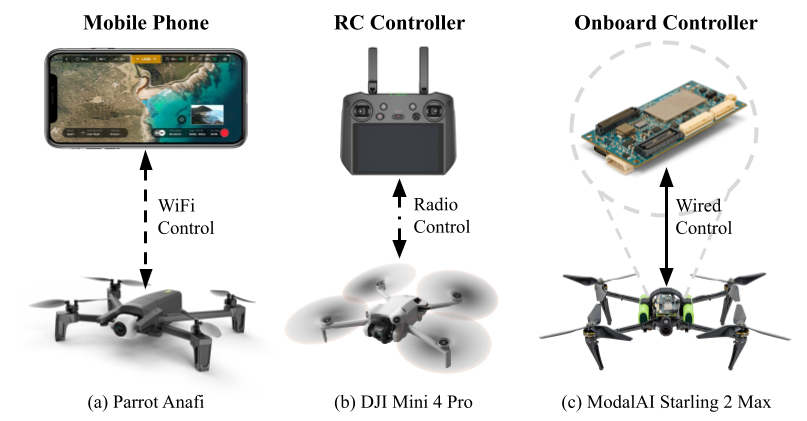
\includegraphics[width=0.85\linewidth]{chapter7/FIGS/control-schemes.png}
    \caption{Drone Control Schemes}
    \label{fig:control-schemes}
\end{figure}

\section{Need for a Hardware-Adaptive Software Architecture}
\label{sec:hardware-adaptive-architecture}
A vital component of SteelEagle is the companion application software which links the edge with the underlying drone hardware and runs mission logic. For the watch prototype, this was an Android application running on-device. For the Onion prototype, this was an application running on the cloudlet that talked to the drone over the network. In both cases, this application served the same role: relay video and telemetry from the drone to the edge, run missions, and send commands to the drone using its SDK.

From the perspective of the backend, the companion application, denoted by the ``Mission'' label, is abstracted behind the data and control servers. This is clear in both the Onion (Figure~\ref{fig:sys-arch-onion}) and watch (Figure~\ref{fig:sys-arch}) architecture diagrams; everything to the right of the data and control server is identical. There is a shared protocol for sending commands on the control plane and for receiving data on the data plane but there are no assumptions made about the makeup of the application. In this way, the companion application represents a kind of drone abstraction layer that enables the drones it interacts with to plug into SteelEagle.

The design of this abstraction layer is difficult. Drones not only have different flight properties, SDKs, and sensors, but also often have divergent control methods, as shown in Figure~\ref{fig:control-schemes}. For instance, some drones may require a radio controller to be connected at all times, even when autonomous commands are sent by an onboard application. Others necessitate a pilot to takeoff manually before autonomous flight can begin. These safeguards can rarely be circumvented without serious modification of the drone hardware, a non-starter for a project focused on accessibility and easy portability.

In addition, the current Parrot Anafi prototype with the Onion payload lacks onboard compute, but this is not the case for all drones. Some have stereo cameras and onboard obstacle avoidance like the Parrot Anafi Ai. A few may even have generalized computation resources like GPUs which could run lightweight versions of the models on the cloudlet. These drones could even support disconnected operation.

The only way to reconcile these differences is to design around them. Ideally, the companion application should be itself highly portable, able to work with many different drones, each using a completely distinct control model. It should take advantage of onboard compute and support disconnected operation. All the while, it must maintain a unified interface for the backend, allowing these drones to gain the benefits of edge-based autonomy.

\begin{figure}
    \centering
    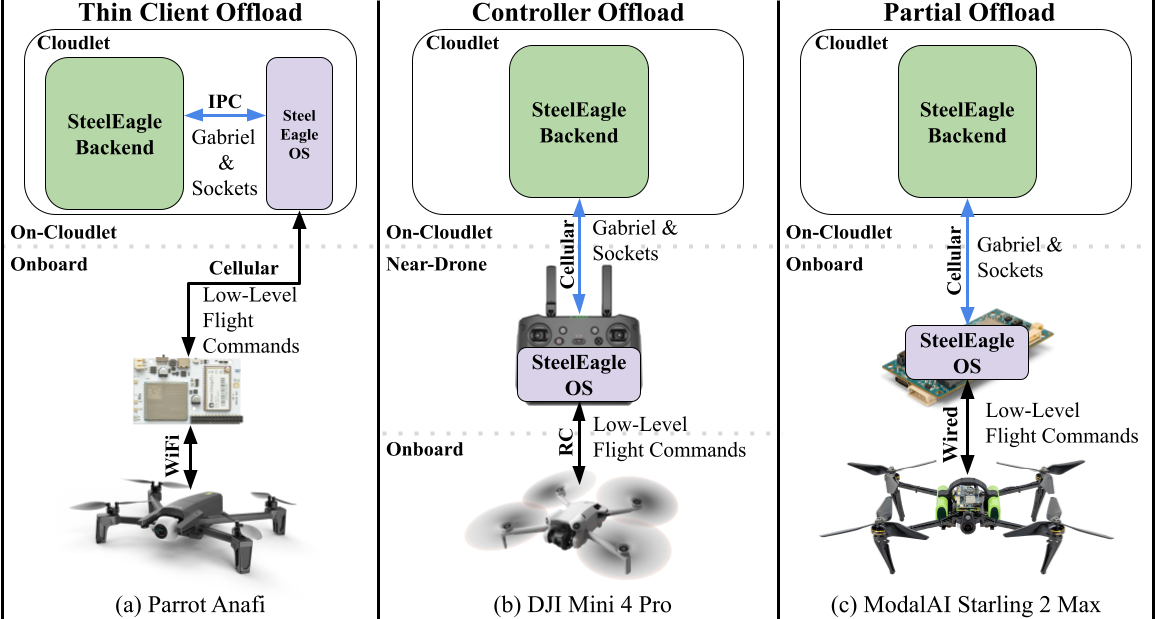
\includegraphics[width=1.0\linewidth]{chapter7/FIGS/hardware-agnostic.png}
    \begin{captext}
    \\[0.2cm] \small The SteelEagle OS can live on the cloudlet, on an RC controller, or on an onboard device. This supports the majority of COTS drone control schemes on the market today.
    \end{captext}
    \caption{SteelEagle OS Placement for Different Control Schemes}
    \label{fig:hardware-agnosticism}
\end{figure}

\section{The SteelEagle Operating System}
\label{sec:companion-operating-system}
To address the above design constraints, it is helpful to view the companion application as the \textit{SteelEagle Operating System}. As with other popular operating systems like Linux, the SteelEagle Operating System (SteelEagle OS) must manage varied underlying hardware (drone control schemes) and run user code (missions). It also has to ensure safe operation via monitoring, interrupts, and permissions. This further motivates separating such an operating system into logical units like the kernel, userspace, memory, and drivers.

\begin{figure}
    \centering
    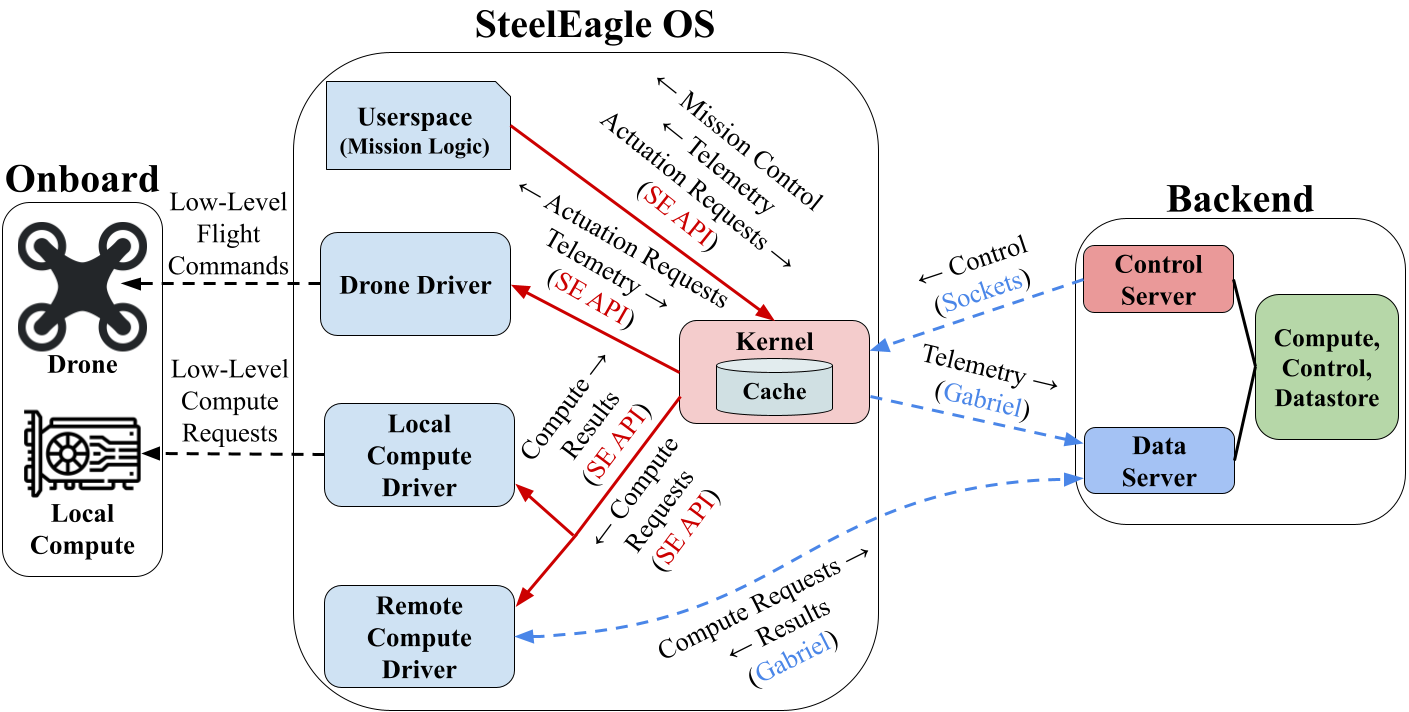
\includegraphics[width=1.0\linewidth]{chapter7/FIGS/companion-os.png}
    \begin{captext}
    \\[0.1cm] \small Dashed connections represent external links, as seen in Figure~\ref{fig:hardware-agnosticism}. All SteelEagle OS modules are assumed to be collocated. The SteelEagle API (shown as SE API) is described in detail in Section~\ref{sec:se-api}.
    \end{captext}
    \caption{Architecture of the SteelEagle OS}
    \label{fig:companion-os}
\end{figure}

The SteelEagle OS architecture, shown in Figure~\ref{fig:companion-os}, is organized in a hierarchical structure, with the kernel acting as the command center, and the userspace and drivers using the kernel for system calls. SteelEagle OS, as illustrated in Figure~\ref{fig:hardware-agnosticism}, can be configured in one of three modes. For a thin client drone (Figure~\ref{fig:hardware-agnosticism}(a)), SteelEagle OS can run on the cloudlet as a proxy with the drone driver talking to the aircraft over cellular. For a RC controller-dependent drone (Figure~\ref{fig:hardware-agnosticism}(b)), SteelEagle OS can run on the RC controller, using native RC to connect to the drone and cellular to communicate with the cloudlet. For a drone with sufficient compute resources onboard (Figure~\ref{fig:hardware-agnosticism}(c)), SteelEagle OS can be deployed onboard, sending commands directly to the drone autopilot over a wired connection while using an onboard modem to communicate with the cloudlet.

All communication between SteelEagle OS modules is done via a unified system call API called the SteelEagle API (shown as the SE API in Figure~\ref{fig:companion-os}) which will be further discussed in Section~\ref{sec:se-api}. This is a near-identical structure to other popular operating systems today. Each driver is designed to interface with one of the pieces of hardware within the overall system. For example, the drone driver is solely responsible for handling all interactions with the physical aircraft and autopilot. There are no constraints on how modules are written, only that it follows the schema of the SteelEagle API. This promotes maximum portability and gives SteelEagle OS the widest possible compatibility umbrella.

There are three primary data flows within SteelEagle OS: the manual control flow (Section~\ref{sec:manual-flow}), the autonomous control flow (Section~\ref{sec:autonomous-flow}), and the computation flow (Section~\ref{sec:computation-flow}). I will step through each flow to show how modules interact with each other. 

\subsection{Manual Control Flow}
\label{sec:manual-flow}
The manual control flow is responsible for giving a remote commander manual control over a drone in case of emergency or in case human assistance is needed. When a commander requests manual control of a drone, a control message is sent from the commander client through the backend over the control server to the SteelEagle OS instance, where it arrives in the kernel module. The kernel is responsible for maintaining this link, and if this link is over the air, its reliability is directly tied to the reliability of the underlying network. 

Once the manual control request arrives at the kernel, it immediately revokes actuation permission from the userspace and prepares for further instructions. Actuation permission gives a module authority to control the drone. The kernel is the only module that always has this permission and it decides when to grant or revoke it for other modules. Any actuation requests received from non-permitted sources are ignored. In this case, if actuation requests arrive from the backend, they are promptly converted into SteelEagle API messages by the kernel, relayed to the drone driver, and executed. Meanwhile, the kernel continues sending telemetry via the data server to the backend which is eventually displayed to the commander client.

\subsection{Autonomous Control Flow}
\label{sec:autonomous-flow}
The autonomous control flow is responsible for running autonomous missions within SteelEagle OS. When a commander sends a mission to a drone, a control message containing compiled mission logic is sent from the commander client through the backend over the control to the kernel. Upon receiving the mission, the kernel sends it to the userspace module and grants the userspace actuation permission.  The sole task of the userspace is to configure, monitor, and run autonomous missions. Once the userspace has the mission, it configures all computation relevant to the mission through the SteelEagle API (Section~\ref{sec:se-api}). For instance, if the mission involves tracking a human target, the userspace may provision an object detector trained for the specified class of human. These messages are sent to the kernel where they are then passed on to the local and remote compute drivers. All compute results will eventually be stored in the kernel cache which can be read by the userspace on demand while it has actuation permission.

As soon as the appropriate computation requests have been acknowledged, the userspace starts the mission. During its lifetime, the mission may actuate the drone by sending SteelEagle API actuation requests, or query computation results by sending SteelEagle API computation requests. All messages are sent to the kernel where they are then delivered to the intended recipient. Fundamentally, this design mirrors the design of the userspace in modern operating systems. Since user code is not trusted, all system-level calls must be validated by the kernel before they are executed. At mission end, the userspace notifies the kernel which then revokes actuation permission and signals an end of mission to the commander.

\subsection{Computation Flow}
\label{sec:computation-flow}
The computation flow is responsible for configuring compute resources and delivering computation results to consumers like the userspace. Computation configuration messages are generated by the userspace during mission setup. These messages, in the case of object detection, contain the model type, camera sensor identification, target class, and confidence score. This will change depending on the task. For example, an obstacle avoidance task may request a MiDaS avoidance model which would be specified with just the model type and camera sensor identification. Regardless, these configuration messages are delivered to the local and remote compute drivers.

After the local and remote compute drivers receive a computation configuration message, they set up the corresponding model, if they have access to it. For the local compute driver, this could be a pruned, less accurate model which can run on constrained mobile hardware. For the remote compute driver, it will request the full size model to be provisioned by the SteelEagle backend. By default, SteelEagle OS attempts to set up appropriate computation resources both locally and remotely. This gives the drone a local fallback model for disconnected operation in case remote resources are inaccessible. As the mission is executed, frames are constantly ferried from the drone driver to the compute drivers via the kernel. There frames are then inferenced using the configured compute, and results are cached on the kernel's datastore. Compute requests sent from the userspace to the kernel can then read these results, indexed by model type.  

\begin{table}[t]
    \centering
    \begin{tabular}{c|c|c|c}
         \textbf{Type} & \textbf{Message} & \textbf{Response} & \textbf{Payload} \\
         \hline
         Telemetry & get\_telemetry & telemetry\_frame & Empty \\
         Telemetry & telemetry\_frame & None & Aircraft telemetry \\
         Telemetry & get\_sensor & sensor\_frame & Sensor ID \\
         Telemetry & sensor\_frame & None & Sensor content \\[0.2cm]

         \hline
         Actuation & actuation\_request & actuation\_ack & Actuation type\textsuperscript{\textdagger} \\
         Actuation & actuation\_ack & None & Success or failure \\[0.2cm]

         \hline
         Compute & compute\_configuration & compute\_ack & Model, sensor, class, confidence \\
         Compute & compute\_request & compute\_result & Model, sensor, class, confidence \\
         Compute & compute\_result & None & Inference result \\[0.2cm]

         \hline
         Mission & mission\_start & mission\_ack & SteelEagle mission \\
         Mission & mission\_stop & mission\_ack & Empty \\
         Mission & mission\_ack & None & Success or failure \\[0.2cm]
         \hline
    \end{tabular}
    \begin{captext}
        \\[0.2cm] \small \textsuperscript{\textdagger}Actuation requests roughly follow the format of the MAVLink API~\cite{MAVLink}. This is the canonical way in which quadrotor drones are controlled. \\
    \end{captext}
    \caption{High-Level Overview of the SteelEagle API}
    \label{tab:unified-api}
\end{table}

\section{SteelEagle API Design}
\label{sec:se-api}
The SteelEagle API forms the backbone of all communication within SteelEagle OS. It is, at its core, a list of synchronous and asynchronous remote procedure calls (RPCs) that modules can invoke on each other. For example, the userspace may make an RPC actuation request to the kernel to move the drone to a GPS location. This request contains the move to GPS actuation type, followed by relevant parameters. In this instance, the parameters would include the target latitude, longitude, and altitude. The actuation request API closely follows the MAVLink API in its overall structure, but drivers can implement the API using a custom SDK of choice~\cite{MAVLink}. Once a request is sent from the userspace to the kernel, it is then forwarded to the drone driver which completes the action and returns an acknowledgment. In this way, modules are easily separable; so long as they communicate using the SteelEagle API, they can be written in any format or language.

RPC calls within the SteelEagle API are divided into four categories: telemetry, actuation, compute, and mission. Telemetry messages are for sending sensor data and the video stream from the drone driver to other customer modules. Actuation messages are for requesting actuation on the drone. Mission control messages relay directives to the userspace from the commander. Compute messages request computation from local or remote engines. Since SteelEagle API RPCs are based on the Protocol Buffer data packaging system, more message types can be added later without breaking compatibility~\cite{Protobuf}. Table~\ref{tab:unified-api} shows a high-level overview of the SteelEagle API and its associated messages.

\section{Implementation Considerations}
As mentioned earlier, portability and flexibility are first class design considerations for SteelEagle OS. For this reason, all OS modules are deployed as containers which can run on a variety of host operating systems. On Linux, Windows, or Mac based hardware, setup is trivial. This covers a broad range of devices, including mobile single-board computers like the Raspberry Pi and most consumer computers. In some cases, the host operating system may not support containers. As a result, SteelEagle OS cannot be set up in its container configuration. Instead, it must be rewritten and optimized for the new environment while maintaining all external abstractions. This is not ideal as it promotes fragmentation of the code base when confronted with incompatible devices. However, this is a necessary concession to ensure SteelEagle can function in almost every case.

If a drone has sensing or actuation capabilities beyond the scope of the SteelEagle API, SteelEagle OS supports freeform RPC calls which can be forwarded from customized mission code to the drone driver. This is similar to \verb|ioctl(2)| in Linux which gives the operating system flexibility when dealing with specialized drivers~\cite{Linux}. Using this system, SteelEagle OS can take advantage of exotic drones without needing to change the SteelEagle API. The API can always be extended later if a critical mass of compatible drones requires this RPC feature. In the case of custom ASICs or local computation, the local compute driver can be written to support any associated API. This is where the language agnosticism of each module becomes advantageous; modules can be written in completely distinct ways as long as they follow their RPC interface. 

\section{Integrating a New Drone into SteelEagle}
\label{sec:new-drone}

The only true test of SteelEagle's drone agnostic design is to successfully integrate a new drone into the system. In this section, I will walk through the integration of the ModalAI Starling 2 Max~\cite{ModalAIStarling2Max}, a drone with completely distinct hardware from the Parrot Anafi series. I will show where development effort needs to be spent and where my design simplifies this task.

\begin{figure}
    \centering
    \vspace{-0.8in}
    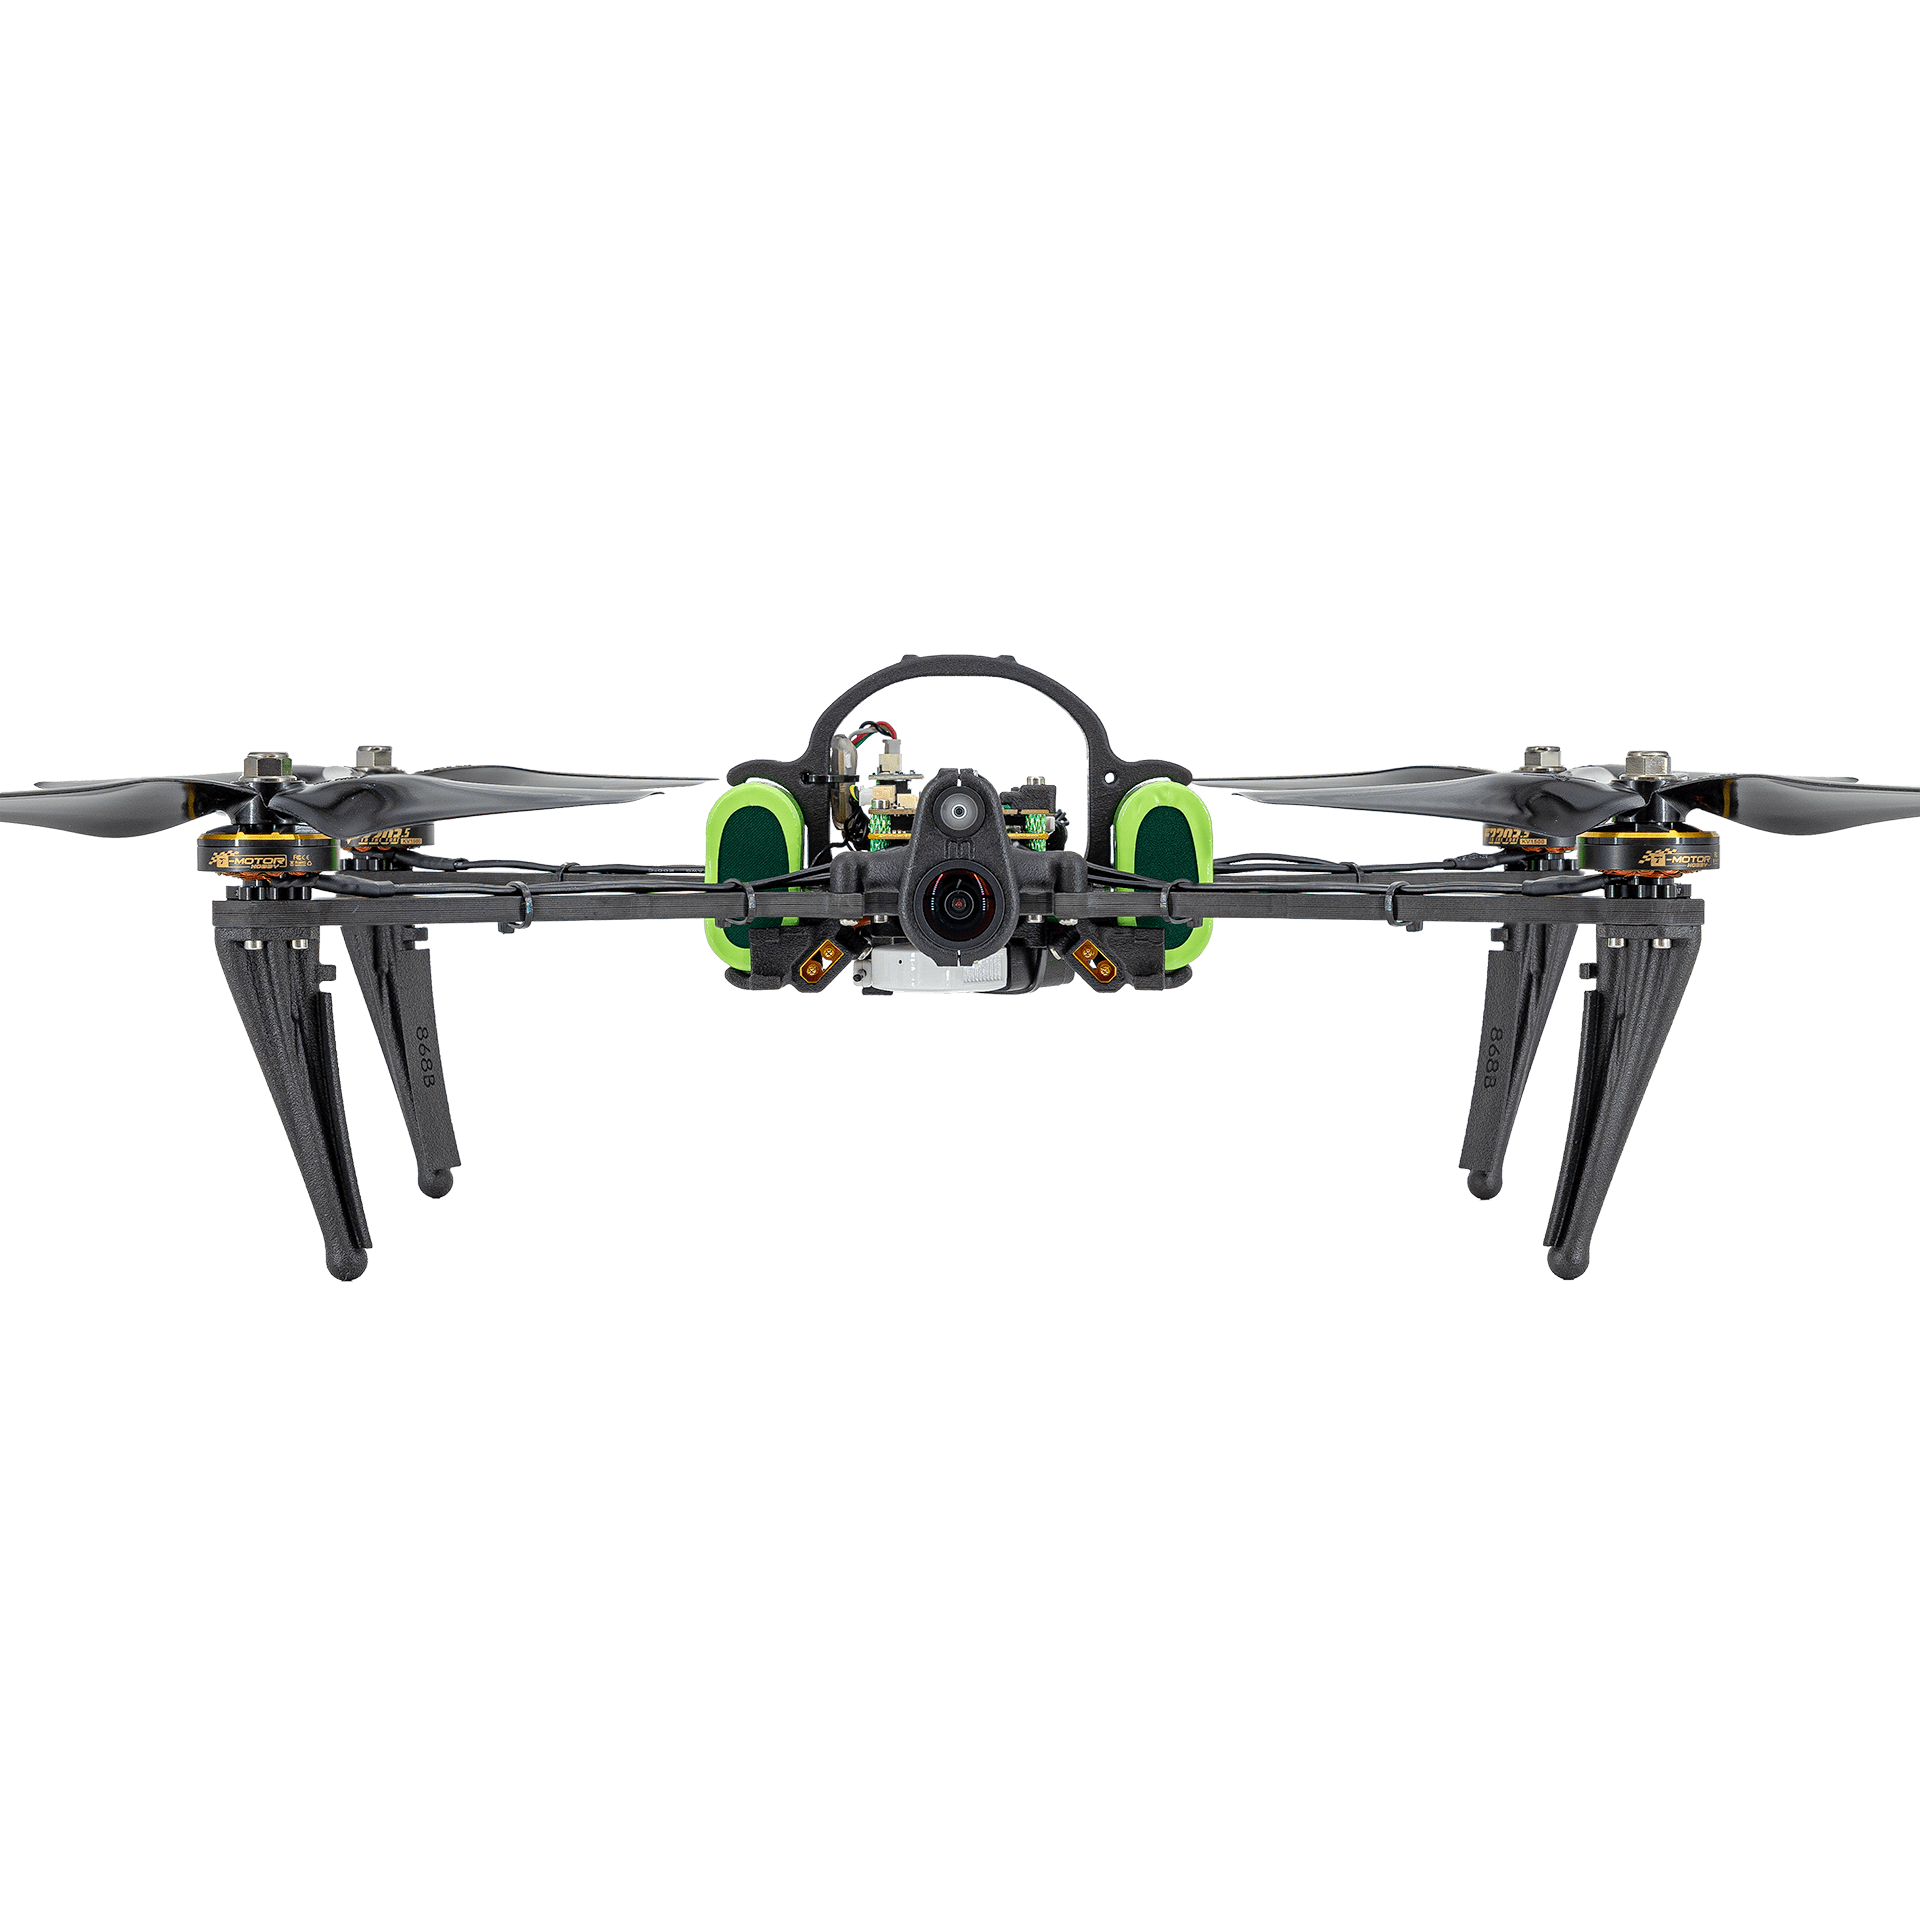
\includegraphics[width=0.6\linewidth]{chapter7/FIGS/starling2max.png}
    \vspace{-0.8in}
    \caption{ModalAI Starling 2 Max~\cite{ModalAIStarling2Max}}
    \label{fig:starling}
\end{figure}

\begin{figure}
    \centering
    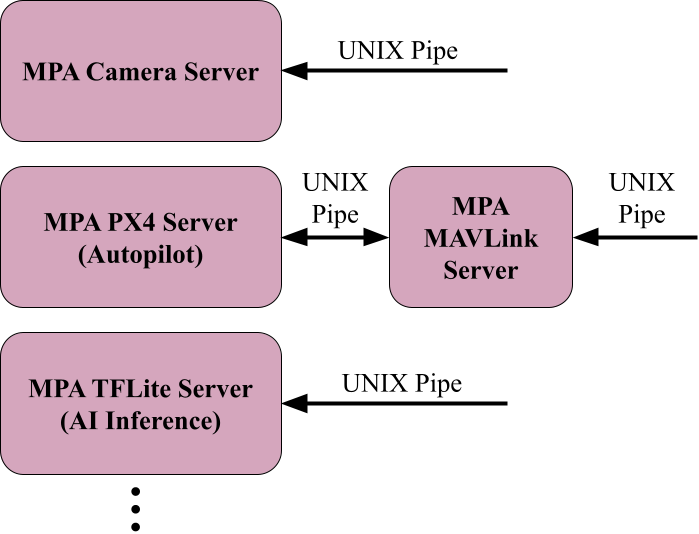
\includegraphics[width=0.5\linewidth]{chapter7/FIGS/mpa.png}
    \begin{captext}
        \\[0.1cm] \small A small selection of the servers avaiable within the default MPA configuration. Each server is started as a UNIX service and can be accessed via UNIX pipes.
    \end{captext}
    \caption{ModalAI Pipe Architecture (MPA) (Adapted from \cite{VOXLSDK})}
    \label{fig:mpa}
\end{figure}

\subsection{Hardware and Software Overview}
The Starling 2 Max, shown in Figure~\ref{fig:starling}, is a quadcopter with a rich sensor suite and significant onboard compute. It is equipped with a downward-facing fisheye visual inertial odometry (VIO) camera for GPS-denied localization, front-facing stereo cameras for obstacle avoidance, and a front-facing RGB camera for perception. Providing onboard intelligence is the VOXL 2 chip, a collaboration with Qualcomm to build a SWaP (size, weight, and power) optimized robotics-focused single-board computer. The VOXL 2 sports a smartphone caliber CPU in the QRB5165, and hosts a proprietary GPU which can inference weight-optimized  models in real time~\cite{VOXL2}. It also has an embedded 4G modem which can communicate with the cloudlet out-of-the-box.

The VOXL runs an Ubuntu~\cite{Ubuntu} distribution and uses standard UNIX services to run its in-flight processes. These services communicate with each other using the ModalAI Pipe Architecture (MPA), an IPC mechanism built on UNIX pipes~\cite{VOXLSDK}. Figure~\ref{fig:mpa} shows a simplified diagram of the MPA. For instance, to send commands to the autopilot, an autopilot service, called the MAVLink service, must first be started. Then, commands can be fed over a UNIX pipe to the service and the drone will actuate.

The VOXL 2 is equipped with PX4 autopilot software which handles all low level flight control~\cite{PX4}. PX4 is a well-known open source autopilot, and it is compatible with the ubiquitous MAVLink protocol~\cite{MAVLink}.

\begin{figure}
    \centering
    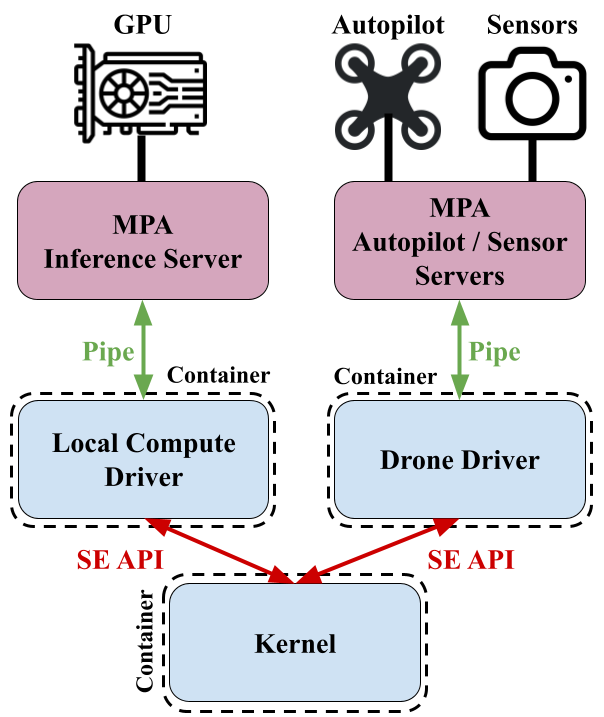
\includegraphics[width=0.4\linewidth]{chapter7/FIGS/voxl-integration.png}
    \begin{captext}
        \\[0.1cm] \small Red arrows show communication using the SteelEagle API. Green arrows show communication using VOXL MPA pipes~\cite{VOXLSDK}.
    \end{captext}
    \caption{VOXL Integration into SteelEagle OS}
    \label{fig:voxl-integration}
\end{figure}

\subsection{Development and Deployment Experience}
There are two main aspects that differentiate the software environment of the Starling from the Parrot Anafi series. First, it has onboard compute and thus requires a compute driver. Second, its control scheme depends on pure MAVLink rather than Parrot Olympe. Thus, a new drone driver and local compute driver must be created. Once this is done, all components of SteelEagle OS can be deployed onboard as Docker containers. Figure~\ref{fig:voxl-integration} shows the integrated system diagram.

\subsubsection{Drone Driver}
As mentioned above, MAVLink is the canonical protocol used to communicate with PX4 autopilots. The MAVLink API is very similar to the Parrot Olympe API; this is not surprising since Olympe is a modified MAVLink wrapper. To convert the existing Olympe driver into a MAVLink driver, only slight modifications are needed.

\subsubsection{Local Compute Driver}
The VOXL 2 has a Tensorflow inference server that can be automatically started on boot. The inference server consumes frames over an MPA pipe and sends out results over a different MPA pipe. A compatible compute driver only needs to transform SteelEagle API compute requests into MPA data to send over the pipe and vice versa. The MPA API is most easily compatible with C/C++ while the rest of SteelEagle OS is written in Python. Thanks to its modular language agnostic design, this is not an issue, and the local compute driver can be written in a different language than the rest of the pipeline without compromising abstraction layers.

\section{Validation}
I have successfully tested the ModalAI Starling 2 Max flying autonomously via SteelEagle both in simulation and in real flight. This proof of concept could be extended to drones running ArduPilot~\cite{Ardupilot} or other drone families like DJI.
